\documentclass[10pt,twocolumn]{article}
\usepackage[letterpaper,margin=0.66in,columnsep=0.23in]{geometry}
\usepackage{times}
\usepackage{microtype}
\usepackage{amsmath,amssymb}
\usepackage{booktabs}
\usepackage{enumitem}
\usepackage{graphicx}
\usepackage{xcolor}
\usepackage{hyperref}
\usepackage{tikz}
\usepackage{balance}
\usetikzlibrary{arrows.meta,positioning}
\setlength{\parindent}{0.75em}
\setlength{\parskip}{0pt}
\setlist{nosep,leftmargin=*}
\hypersetup{colorlinks=true,linkcolor=black,citecolor=black,urlcolor=blue}
\newcommand{\taskname}{\textit{Text-Conditioned Visual Complementarity Localization}}

\begin{document}
\twocolumn[
\begin{center}
\vspace{-0.37in}
{\fontsize{16}{18}\selectfont\bfseries
What Does the Image Add? Text-Conditioned Localization of Complementary Visual Information\par}
\vspace{0.45em}
{\small CSCI-GA 2271 Computer Vision \hspace{1.0em} Fall 2026 Project Proposal\par}
\vspace{0.28em}
{\small\bfseries Track: Agent Track \hspace{1.4em} Format: Research Project\par}
\vspace{0.58em}
\end{center}
]

\begin{abstract}
Vision-language models such as CLIP are commonly interpreted by asking which image regions support an image-text similarity score or prediction. We study a different question: \emph{given the paired text, which regions of the image contain semantic information that the text has not already covered?} We formulate \taskname{} as a region-level, text-conditioned interpretability task. Our method assigns each image region a complementarity score and is trained and evaluated using controlled text interventions: when a visual detail is added to the caption, the score of the corresponding region should decrease while unrelated regions remain stable. Flickr30K Entities provides grounded phrase-box correspondences for a controlled benchmark; Visual Genome provides a second, denser testbed. We will compare against similarity, gradient, decomposition, and masking-based CLIP explanations. The core contribution is a new interpretability target and intervention-based verification protocol, not a finance-specific predictor. If time and data access permit, financial news will serve only as a real-world downstream testbed for whether complementary visual content can matter outside standard benchmarks.
\end{abstract}

\section{Problem, Significance, and Research Questions}
Contrastive vision-language pretraining aligns matched images and text in a shared representation space \cite{radford2021}. Existing interpretation methods can localize image patches that contribute to a CLIP representation or matching score \cite{gandelsman2024,zhao2026}, while recent masking methods identify concept regions that are important for a prediction \cite{agarwal2026}. However, \emph{importance} and \emph{complementarity} are not the same. A dog region may be crucial for matching the caption ``a man with a dog'' but provide little information beyond the text because the dog is already mentioned. Conversely, an unmentioned fire truck may contribute little to the current matching score while containing substantial visual information not stated in the caption.

This distinction matters because natural captions are incomplete by design. Prior work has shown that CLIP does not naturally distinguish captions that complement an image from descriptions that replace it \cite{zur2024}, and CIEA shows that preserving image information beyond paired text can improve multimodal retrieval \cite{zeng2025}. Yet these works do not directly provide a spatial answer to the question ``where is the information the text has not covered?''

We therefore study three questions:
\textbf{RQ1:} Can we define and learn a region-level score $C(r_k\mid T)$ that estimates how much semantic content in region $r_k$ remains uncovered by paired text $T$?
\textbf{RQ2:} Does this score respond correctly to controlled changes in the text, decreasing specifically when the missing visual detail is added?
\textbf{RQ3:} Does the resulting complementarity map generalize across datasets and vision-language encoders, and does it capture a different explanatory signal from ordinary saliency or region importance?

\textbf{Proposed novelty.} We do not claim that complementary multimodal information, spatial CLIP interpretation, or text intervention is individually new. Our contribution is their combination into a specific interpretability target: \emph{region-level, text-conditioned visual complementarity}, together with a locality-constrained intervention test that can falsify the explanation. CIEA extracts complementary features for retrieval \cite{zeng2025}; CLIP decomposition, Grad-ECLIP, and CCI explain spatial evidence or importance \cite{gandelsman2024,zhao2026,agarwal2026}; Counterfactual Phrase Intervention (CPI) measures phrase sensitivity for pretraining data selection \cite{go2026}. Our task instead asks whether a visual region is informative \emph{because its semantics are not yet present in the paired text}.

\section{Related Work}
\textbf{Vision-language representation.} CLIP learns a shared image-text space using contrastive learning \cite{radford2021}. This makes text a natural interface for probing visual representations, but global similarity does not identify which visual semantics are omitted from a particular caption.

\textbf{Spatial interpretation of CLIP.} Gandelsman et al. decompose CLIP's image representation over patches, layers, and attention heads and uncover emergent spatial localization \cite{gandelsman2024}. Grad-ECLIP produces image and word heatmaps explaining a specific CLIP matching result \cite{zhao2026}. CCI clusters CLIP patch embeddings into coherent concept regions and measures importance by masking them, achieving strong faithfulness on retrieval benchmarks \cite{agarwal2026}. These methods answer which regions support a representation or decision, not whether those regions contain information redundant with or complementary to the paired text.

\textbf{Complementarity and interventions.} CIEA explicitly extracts visual information complementary to text to improve multimodal retrieval \cite{zeng2025}. Zur et al. distinguish captions from fuller image descriptions and show that standard CLIPScore does not capture this distinction well \cite{zur2024}. CPI uses controlled phrase substitution to measure whether individual caption phrases materially affect image-text alignment, but its target is phrase-sensitive data curation rather than spatial complementarity localization \cite{go2026}. Visual Credit Audit asks whether a multimodal decision receives additional support from an image beyond text-only controls, but operates at the whole-image decision level rather than localizing which visual region contributes uncovered semantics \cite{liu2026vca}. These works motivate our use of intervention as a verification tool.

\section{Method}
\subsection{Task Definition and Regions}
Given image $I$, paired text $T$, and candidate visual regions $\{r_k\}_{k=1}^{K}$, we seek a score
\begin{equation}
q_k = C_\theta(r_k\mid T) \in [0,1],
\end{equation}
where a high value means that region $r_k$ contains visually grounded semantics that are not adequately covered by $T$. We use \emph{complementarity} as an operational, intervention-defined quantity rather than claiming an exact information-theoretic mutual-information decomposition. In the controlled benchmark, regions come from ground-truth Flickr30K Entities boxes. We will later test model-generated regions from CCI-style patch clustering or GroundedSAM to remove dependence on annotations.

A frozen vision-language encoder produces a region feature $v_k$ and text feature $t$. The primary model is a small scorer
\begin{equation}
q_k = g_\theta([v_k,t,v_k\odot t,|P_vv_k-P_tt|]),
\end{equation}
where $P_v$ and $P_t$ are learned projections when the feature dimensions differ. The scorer is intentionally lightweight so that the research focus remains on the interpretability objective rather than large-scale model training.

\subsection{Controlled Text Intervention}
Flickr30K Entities links caption phrases to image boxes, allowing us to construct intervention pairs for a target region $r_k$ and phrase $p_k$ \cite{plummer2017}. Let $T^{+}$ explicitly cover $p_k$, while $T^{-}$ omits or generalizes that detail. The core constraint is
\begin{equation}
q_k(I,T^{-}) > q_k(I,T^{+}).
\end{equation}
We train with a margin-ranking loss
\begin{equation}
\mathcal L_{rank}=\max(0,m-q_k(I,T^{-})+q_k(I,T^{+})).
\end{equation}
To enforce locality, an intervention about $r_k$ should minimally change scores of unrelated regions:
\begin{equation}
\mathcal L_{loc}=\frac{1}{K-1}\sum_{j\neq k}|q_j(I,T^{-})-q_j(I,T^{+})|.
\end{equation}
We will add a matched-control loss using captions in which a non-target phrase is changed. The full objective is $\mathcal L=\mathcal L_{rank}+\lambda_{loc}\mathcal L_{loc}+\lambda_{ctrl}\mathcal L_{ctrl}$.

Intervention generation is a major validity concern. We will use three levels of control: (i) deterministic phrase removal/generalization, (ii) matched edits that preserve length and syntax as closely as possible, and (iii) natural multi-caption pairs for the same image when one caption mentions a grounded entity or attribute and another does not. Agent-assisted candidate edits may be used in the Agent Track, but they will be automatically checked for target coverage and manually audited on a stratified sample; failures will be documented in the Agent Log.

\begin{figure}[t]
\centering
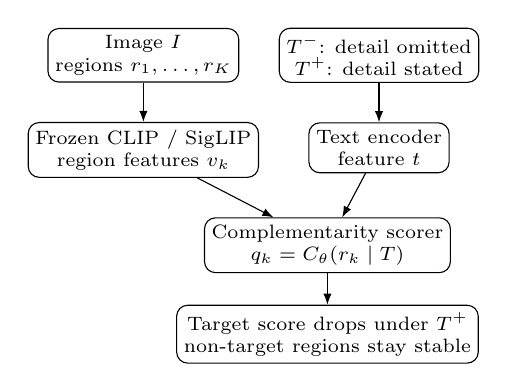
\begin{tikzpicture}[node distance=3.0mm, every node/.style={font=\scriptsize}, box/.style={draw,rounded corners,align=center,inner sep=2.6pt}, arr/.style={-{Latex[length=1.4mm]},thin}]
\node[box] (img) {Image $I$\\regions $r_1,\ldots,r_K$};
\node[box,right=5mm of img] (text) {$T^{-}$: detail omitted\\$T^{+}$: detail stated};
\node[box,below=5mm of img] (enc) {Frozen CLIP / SigLIP\\region features $v_k$};
\node[box,below=5mm of text] (tenc) {Text encoder\\feature $t$};
\node[box,below right=5mm and -7mm of enc] (score) {Complementarity scorer\\$q_k=C_\theta(r_k\mid T)$};
\node[box,below=4mm of score] (verify) {Target score drops under $T^{+}$\\non-target regions stay stable};
\draw[arr] (img)--(enc); \draw[arr] (text)--(tenc);
\draw[arr] (enc)--(score); \draw[arr] (tenc)--(score); \draw[arr] (score)--(verify);
\end{tikzpicture}
\caption{Core idea: complementarity is text-conditioned and must change locally under a controlled caption intervention.}
\label{fig:overview}
\vspace{-1mm}
\end{figure}

\section{Experiments and Evaluation}
\textbf{Primary benchmark.} Flickr30K Entities contains 31,783 images, 158,915 captions, and 276k manually annotated bounding boxes linked to caption phrases \cite{plummer2017}. It is well suited to controlled region-text interventions. We will split intervention templates and images by the official train/validation/test partitions to prevent leakage.

\textbf{Generalization benchmark.} Visual Genome provides dense region descriptions, boxes, objects, attributes, and relations \cite{krishna2017}. We will use it to test whether a scorer trained on Flickr30K Entities transfers to a denser vocabulary and different annotation style.

\textbf{Baselines.} We will compare against (i) random and region-area controls; (ii) inverse region-text cosine similarity; (iii) Gandelsman-style patch contribution; (iv) Grad-ECLIP saliency aggregated over regions; and (v) CCI masking importance. If implementation time permits, we will also compare to a CIEA-inspired complementary feature score. The key question is whether these existing importance or similarity signals satisfy our intervention-specific tests without being trained for complementarity.

\textbf{Metrics.} Our primary metric is the \emph{Target Intervention Gap}
\begin{equation}
\mathrm{TIG}=q_k(I,T^{-})-q_k(I,T^{+}),
\end{equation}
which should be positive and large for the targeted region. \emph{Off-Target Stability} measures the mean absolute score change over $j\neq k$ and should be small. With ground-truth regions, we report target-region ranking Accuracy@1 and MRR; with free-form masks, we report pointing accuracy and IoU against the grounded box. We also report deletion faithfulness by masking high-complementarity regions and measuring loss of recoverability for the omitted phrase. Results will be averaged over multiple seeds with confidence intervals where practical.

\textbf{Ablations.} We will test ground-truth boxes versus model-generated regions, CLIP versus SigLIP, crop features versus pooled patch features, each loss term, different intervention constructions, and training on one dataset versus transfer to the other. A critical negative control edits an unrelated caption phrase; a valid complementarity method should not move the target region score substantially.

\textbf{Optional real-world testbed.} Only after the core CV method is validated, we will apply it to paired financial-news images and headlines. The existing Sina corpus provides a ready testbed; licensed WSJ data will be used only if access is available. The finance experiment is not required for the method to succeed and is not the source of the novelty. It asks whether regions identified as visually complementary to a headline correspond to externally meaningful signals such as volatility, volume, or attention after controlling for text and visual sentiment.

\section{Deliverables, Risks, Verification, and Timeline}
\textbf{Expected deliverables.} (1) A reproducible benchmark builder for text-conditioned region interventions; (2) a complementarity scorer and visualization pipeline; (3) implementations of strong spatial-interpretability baselines; (4) quantitative evaluation on Flickr30K Entities and Visual Genome; (5) ablations and qualitative failure analysis; (6) code repository with incremental commits and a research-paper-style final report; and (7) the required Agent Log. The optional finance testbed is an extension rather than a core deliverable.

\textbf{Risks and fallbacks.} The largest risk is that the model exploits textual shortcuts rather than visual complementarity. We address this with matched edits, unrelated-edit controls, natural multi-caption pairs, and manual audits. Region granularity may also confound results; we therefore begin with human boxes before testing CCI/GroundedSAM regions. If the learned scorer does not beat simple inverse similarity, the project will still produce a controlled benchmark and a systematic falsification analysis explaining when existing attribution signals do or do not measure complementarity, but the primary goal is to demonstrate a measurable gain on intervention consistency and locality.

\textbf{Agent Track verification.} Agent tools may assist with literature search, boilerplate code, experiment scripting, caption-edit candidates, and report/figure preparation. We will independently verify generated code through unit tests and small hand-checked examples, reproduce key baseline behaviors before extension, audit intervention data, rerun core experiments across seeds, and maintain an Agent Log emphasizing incorrect suggestions, implementation failures, and how each result was verified. Every team member will be prepared to explain any submitted code during the final walkthrough.

\textbf{Compute.} Frozen CLIP/SigLIP inference and a small scorer are expected to fit on a single modern GPU. NYU HPC or Google Cloud credits will be used for feature extraction, multi-backbone ablations, and repeated runs. The design intentionally avoids training a foundation model from scratch.

\textbf{Preliminary timeline.} Weeks 1--2: data pipeline, CLIP features, and reproduction of attribution baselines. Weeks 3--4: controlled intervention benchmark and shortcut audits. Weeks 5--7: scorer, ranking/locality objectives, and core Flickr30K experiments. Weeks 8--9: CCI/GroundedSAM regions and Visual Genome transfer. Weeks 10--11: full ablations, faithfulness tests, and multiple seeds. Week 12: optional financial-news testbed. Weeks 13--14: failure analysis, final report, poster/presentation, code walkthrough preparation, and Agent Log.

\balance
\vspace{0.5mm}
{\footnotesize
\begin{thebibliography}{10}
\setlength{\itemsep}{0.5pt}
\bibitem{radford2021} A. Radford et al. ``Learning Transferable Visual Models From Natural Language Supervision.'' \emph{ICML}, 2021. \href{https://proceedings.mlr.press/v139/radford21a.html}{[link]}
\bibitem{gandelsman2024} Y. Gandelsman, A. Efros, and J. Steinhardt. ``Interpreting CLIP's Image Representation via Text-Based Decomposition.'' \emph{ICLR}, 2024. \href{https://proceedings.iclr.cc/paper_files/paper/2024/hash/5085a2b8c298edeadc46b9ffe6df5f64-Abstract-Conference.html}{[link]}
\bibitem{zur2024} A. Zur et al. ``Updating CLIP to Prefer Descriptions Over Captions.'' \emph{EMNLP}, 2024. \href{https://aclanthology.org/2024.emnlp-main.1125/}{[link]}
\bibitem{zeng2025} D. Zeng et al. ``Enhancing Multimodal Retrieval via Complementary Information Extraction and Alignment.'' \emph{ACL}, 2025. \href{https://aclanthology.org/2025.acl-long.1073/}{[link]}
\bibitem{zhao2026} C. Zhao et al. ``Grad-ECLIP: Gradient-based Visual and Textual Explanations for CLIP.'' \emph{IEEE TPAMI}, 2026. \href{https://doi.org/10.1109/TPAMI.2026.3714444}{[link]}
\bibitem{agarwal2026} A. Agarwal, S. Karanam, and V. Gandhi. ``Concept Regions Matter: Benchmarking CLIP with a New Cluster-Importance Approach.'' \emph{CVPR}, 2026. \href{https://openaccess.thecvf.com/content/CVPR2026/html/Agarwal_Concept_Regions_Matter_Benchmarking_CLIP_with_a_New_Cluster-Importance_Approach_CVPR_2026_paper.html}{[link]}
\bibitem{go2026} H. Go, S. Lee, and H. Choi. ``What Does the Caption Really Say? Counterfactual Phrase Intervention for Compositional Data Selection in Vision-Language Pretraining.'' arXiv:2605.22651, 2026. \href{https://arxiv.org/abs/2605.22651}{[link]}
\bibitem{liu2026vca} F. Liu et al. ``Visual Credit Audit for Multimodal Spatial Reasoning.'' arXiv:2607.27069, 2026. \href{https://arxiv.org/abs/2607.27069}{[link]}
\bibitem{plummer2017} B. Plummer et al. ``Flickr30K Entities: Collecting Region-to-Phrase Correspondences for Richer Image-to-Sentence Models.'' \emph{IJCV}, 2017. \href{https://arxiv.org/abs/1505.04870}{[link]}
\bibitem{krishna2017} R. Krishna et al. ``Visual Genome: Connecting Language and Vision Using Crowdsourced Dense Image Annotations.'' \emph{IJCV}, 2017. \href{https://link.springer.com/article/10.1007/s11263-016-0981-7}{[link]}
\end{thebibliography}
}
\end{document}
